\documentclass[12pt]{exam}

% LOAD PACKAGES
\usepackage{amsmath} % allows for align env and other things
\usepackage{amssymb} % 
\usepackage{mathtools} % allows for single apostrophe
\usepackage{enumitem} % allows for alpha lettering in enumerated lists
\usepackage{lastpage}
\usepackage{array} % for table alignments
\usepackage{graphicx} % if images are needed

\addpoints

% Initials
\newcommand{\Initials}{\textit{\Course, \TestName. Your initials: \underline{\hspace{3cm}}} \vspace{1pt}}
\newcommand{\InitialsLeft}{\noindent \hspace{-18pt}\textit{\Course, \TestName. Your initials: \underline{\hspace{3cm}}} \vspace{1pt}}
\newcommand{\InitialsRight}{\begin{flushright}\textit{\Course, \TestName. Your initials: \underline{\hspace{3cm}}} \vspace{1pt}\end{flushright}}


% INSTRUCTIONS FOR DISTANCE LEARNING COURSES: PROCTORS/FACILITATORS
\newcommand{\InstructionsDistanceProctors}{\begin{itemize}

    \item A proctor/facilitator is required to be present while the student is taking this test.
    
    \item A proctor/facilitator must connect with the on-campus class during this test.   
        
    \item For any connection help: gtonlinesupport@pe.gatech.edu
    
    \item No communication is allowed among students taking the exam.

\end{itemize}}


% INSTRUCTIONS FOR DISTANCE LEARNING COURSES: STUDENTS
\newcommand{\InstructionsDistanceStudents}{\begin{itemize} \setlength\itemsep{.15em}
    
    % \item If there are questions during the exam, students can call/text \InstructorContact, at \InstructorNumber, under supervision of their proctor/facilitator.     
        
    \item {\bf Show your work} and justify your answers for all questions unless stated otherwise.

    \item You will have \Duration continuous minutes (no breaks) to take the exam. 
    
    \item There are \Points total points possible.

    \item Calculators, notes, cell phones, books are not allowed.
    
    \item Please write your answers neatly and show all of your work. 
    \item Use dark and clear writing: your exam will be scanned into a digital system.
    
    \item Exam pages are double sided. Be sure to complete both sides. 
    
    \item Leave a 1 inch border around the edges of exams.
    
    \item Check that every page has the same booklet number.

\end{itemize}}


% INSTRUCTIONS FOR DISTANCE LEARNING COURSES: STUDENTS
\newcommand{\InstructionsCovid}{\begin{itemize} \setlength\itemsep{.15em}
    
    \item If there are questions during the exam, students can email their instructor or message them through Canvas. 
    
    % \InstructorContact, at \InstructorNumber, under supervision of their proctor/facilitator.     
        
    \item {\bf Show your work} and justify your answers for all questions unless stated otherwise.

    \item You will have \Duration continuous minutes (no breaks) to take the exam. 
    
    \item There are \Points total points possible.
    
    \item Your work must be your own. Please do not communicate with anyone other than the instructor during the exam. Otherwise, students can use any resources available to them the answer the questions that are given. 
    
    \item Students can take this exam at home.
    
    \item Please write your answers neatly and show all of your work. 
    
    \item Students should scan their work and submit it through Canvas. There should be an \textbf{assignment} in Canvas for this exam. The process for submitting your work will be similar to what you have used for homework. 
    
    \item Work must be submitted today by 12:30 ET. 
    
    \item Please use dark and clear writing so that the scan is easy to read. 
    
    \item Please write your name or initials at the top of every page and solve the questions in the exam in the order they are given. 
    
    \item There is no need to print the exam at home. As long as you solve problems in the order they are given (just like the written homework sets), you can write out your work on your own paper. But of course, you can print the exam out if you prefer and write your answers on the printed copy. 
    
    \item Please upload your work as a single PDF file. If this is not possible you can email your work to your instructor. 


    
\end{itemize}}

% FANCY HEADERS - MAKE EMPTY
\pagestyle{headandfoot}
\runningfooter{}{}{}


% ADJUST MARGINS FOR DISTANCE LEARNING REQUIREMENTS
\usepackage[tmargin=1.7in,bmargin=1.05in,left=1in,right=1in]{geometry}


% TIKZ DIAGRAMS
\usepackage{color}
\usepackage{tikz}  \usetikzlibrary{arrows} 
\usetikzlibrary{calc} 


% ADJUST FIRST LINE IN PARAGRAPH INDENTATION 
\setlength\parindent{0pt}


% COURSE SPECIFIC INFORMATION
\newcommand{\Course}{Math 2552}
\newcommand{\Semester}{Spring}
\newcommand{\Year}{2020}
\newcommand{\Instructors}{Dr. Greg Mayer}

% WHO TO CONTACT DURING EXAM IF QUESTIONS
\newcommand{\InstructorContact}{Dr. Greg Mayer}


\usepackage{spalign} % Joe Rabinoff's matrix package

\newcommand{\LastPage}{\begin{center}\textit{This page may be used for scratch work. Please indicate clearly if you would like your work on this page to be graded. }\end{center}   }

\newcommand{\Scratch}{\begin{center}\textit{This page may be used for scratch work for the previous question. Your proctor should scan this page whether it is used or not. }\end{center}   }


% DERIVATIVES
\newcommand{\dydt}{{\frac{dy}{dt}}} % 
\newcommand{\dydx}{{\frac{dy}{dx}}} % 
\newcommand{\dydtt}{{\frac{d ^2y}{dt^2}}} % 
\newcommand{\dydxx}{{\frac{d^2y}{dx^2}}} % 
\newcommand{\dydttt}{{\frac{d^3y}{dt^3}}} % 

\newcommand{\ddt}{{\frac{d}{dt}}} % 
\newcommand{\ddx}{{\frac{d}{dx}}} % 
\newcommand{\dudt}{{\frac{du}{dt}}} % 
\newcommand{\dvdx}{{\frac{dv}{dx}}} % 
\newcommand{\dxdt}{{\frac{dx}{dt}}} % 
\newcommand{\dxdtt}{{\frac{d^2x}{dt^2}}} % 
\newcommand{\dzdt}{{\frac{dz}{dt}}} % 



% TEST SPECIFIC INFORMATION
\newcommand{\TestName}{Midterm 2A}
\newcommand{\TestDate}{June 2019}
% \newcommand{\TestTime}{} % QUP
\newcommand{\TestTime}{10:05 am to 11:20 am}
\newcommand{\Duration}{75  }
\newcommand{\Points}{50 }


\begin{document}
    
\input{../CMCoverPage}

\newpage \InitialsRight

% QUP EXAM
\begin{questions}

    \question[10] 
    Use the method of reduction of order to find a second solution, $y_2$, to the DE so that $\{y_1,y_2\}$ forms a fundamental set. $$ y'' - \frac 1t y' + \frac{1}{t^2}y = 0, \quad t>0, \quad y_1(t) = t$$


    \newpage \InitialsLeft \\ \Scratch 

    
    \newpage    \InitialsRight
    
        \question[9] Consider the system of equations. 
        $$
        x_1 ' = 3x_1 -2x_2 + 4x_3, \qquad x_2 ' = -2x_1 + 6x_2 + 2x_3 , \qquad x_3 ' = 4x_1 + 2x_2 + 3x_3 
        $$
        \begin{enumerate} 
            \item[a)] Express the system of equations in the form $\vec x \, ' = A \vec x$. \vspace{3cm} 

            \item[b)] Determine the eigenvectors of $A$ and write down the general solution. You may use that the only eigenvalues of $A$ are $7$ and $-2$. 
                
        \end{enumerate}
        
    \newpage \InitialsLeft
    \Scratch 
        

    \newpage \InitialsRight
    
    \question[10] A 4 kg mass stretches a spring 0.1 meters. The mass is pushed upward, contracting the spring a distance of 0.1 meters, and then set in motion with a downward velocity of 2 m/s. There is no damping. 
    \begin{parts} \part[6] Solve the IVP. You may use that the acceleration due to gravity is $g = 10$ m/s$^2$. \vspace{9cm} \part[1] What is the frequency of the motion? It is not necessary to specify units. \vspace{1cm} \part[3] Sketch the phase portrait for this system. Include the trajectory, $\vec r(t)$, in the phase portrait that corresponds to the initial conditions. Clearly label this trajectory and do not forget to label your axes.  \end{parts} 

    \newpage \InitialsLeft

    \question[2] Determine all values of $\alpha$, if any, for which all solutions tend to zero as $t\to\infty$. $$y'' - (2\alpha - 1) y' + (\alpha^2-\alpha+1) y = 0, \quad \alpha \in \mathbb R$$ \vspace{5cm}  % 4.3.47
    
    
    % \question[2] % 6.3.4
    % State the largest possible interval on which solutions to the IVP are certain to exist. Do not solve the DE.  $$(t-2)y'''+ty''+5t^2y'+2t^3y = \ln t, \quad y(1) = 1$$. \vspace{3cm}
    
    \question[3] Consider a one-dimensional lattice consisting of $3$ lattice points, as in the figure.
    
        \begin{center}
            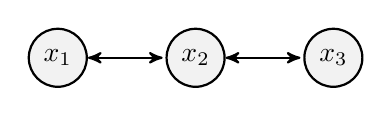
\begin{tikzpicture}
                \begin{scope}[<->,>=stealth',shorten >=1pt,auto,node distance=1.75cm,thick, main node/.style={circle,fill=gray!10,draw}]
                \node[main node] (1) {$x_1$};
                \node[main node] (2) [right of=1] {$x_2$};
                \node[main node] (3) [right of=2] {$x_3$};
                \path[every node/.style={font=\sffamily\small}]
                (1) edge node[below] {} (2)
                (2) edge node [above] {} (3);
                \end{scope}
            \end{tikzpicture}  
        \end{center}  
        
        Let $x_j(t)$ be the number of particles residing at the $j$th lattice point at time $t$. Assume that $x_j$ satisfies the following rate equations.
        \begin{align*} 
            \frac{dx_1(t)}{dt} = k(x_2 - x_1) , \quad 
            \frac{dx_2(t)}{dt} = k(x_3 - 2 x_2 + x_1 ) , \quad 
            \frac{dx_3(t)}{dt} = kx_2 
        \end{align*} 
        Assume $k \in \mathbb R$, $k \ne 0$, and $t \ge 0$. Determine whether the total number of particles in the system is constant. 


    \newpage \InitialsRight
    \question[6]  Determine a suitable form for the particular solution, $Y(t)$, to the differential equations if the method of undetermined coefficients is to be used. Do not determine the values of the coefficients or solve the differential equations. 
    \begin{parts}
        \part $y'' + 4y = t^2 + \sin(2t)$ \vspace{8cm}
        \part $y'' +2y' - 3y = 3te^t\sin t$
    \end{parts} 

    \newpage \InitialsLeft


    \question[10] Use variation of parameters to identify the general solution to $$t^2 y'' - t(t+2)y' + (t+2)y = 5t^3, \quad t > 0$$ Solutions to the corresponding homogeneous equation are $y_1(t) = t$, $y_2(t) = te^t$.
    

    
    
\end{questions}
    
\newpage \LastPage 


\end{document}

